\newpage

\section{Tracer des courbes et surfaces en Python}\index{courbesPython}

\subsection{Pour bien commencer}

Vous devrez utiliser \emph{Pyzo} pour exécuter votre code Python. \emph{Pyzo} est un éditeur de programme léger permettant d'exécuter du code Python. 

Ouvrir l'éditeur \emph{Pyzo} en cliquant d'abord sur l'icône 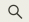
\includegraphics[width=1cm]{./images/activite7/icone_recherche} puis en complétant la barre de recherche : 

\uneimageici{./images/activite7/recherche_pyzo.png}{.5\textwidth} % reprise image existante

\emph{Pyzo} s'ouvre et vous propose deux zones distinctes de travail :
\begin{itemize}
\item à gauche l'éditeur dans lequel vous allez taper votre code,
\item à droite la console dans laquelle vont apparaître les erreurs de code et les résultats fournis après avoir exécuté le code Python.
\end{itemize}

\uneimageici{./images/activite7/ecran_pyzo.png}{.8\textwidth}% reprise image existante

Commencez par créer un nouveau fichier. Pour cela, sélectionner \texttt{Nouveau} dans le menu \texttt{Fichier}

\uneimageici{./images/activite7/nouveau_fichier.png}{.4\textwidth} % reprise image existante

Puis enregistrez votre fichier au format \texttt{Nom-date.py}

